\scanpage{19}
des fibres $I_\alpha$ et $\widetilde A_\alpha$ de $I$ et $A$ au dessus de $\alpha$. La donnée d'une courbe standart $G$ épinglée sur $\mathcal S$ équivaut à la donnée, \deleted{de} pour \unsure{tt|$\forall$} $\alpha\in S$, d'une courbe relative (propre lisse \inserted{rel\textsuperscript{t}} $\unsure{6|0}$-connexe) $Y_\alpha$ \unsure{sur} $\mathcal S$, de genre relatif $g_\alpha$, \uline{et} d'un \inserted{$\mathcal S$-}mono. $(\widehat I_\alpha)_{\mathcal S}\hookrightarrow Y_\alpha$.

Désignons, \deleted{par $\mathcal M_{g_\alpha,\deleted{\nu_\alpha}\inserted{\unsure{\widehat I_\alpha|\widehat I}}}$} pour \deleted{\unsure{deux|de}}\inserted{un} entier naturel $g\deleted{\unsure{\alpha|\nu}}$ et un ens. fini $I$ (de cardinal $\nu$) par
\figure{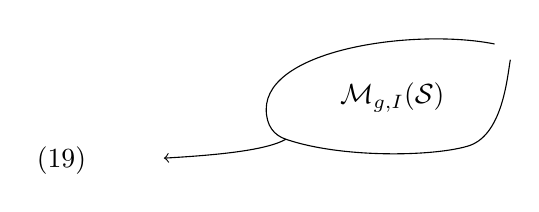
\begin{tikzpicture}[baseline=(m.base)]
\node (m) at (0,0) {$\mathcal M_{g,I}(\mathcal S)$};
\draw (1.3,.68) .. controls (.3,.88) and (-1.6,.62) .. (-1.6,-.15)
 .. controls (-1.6,-.36) and (-1.5,-.48) .. (-1.35,-.53)
 .. controls (-.65,-.77) and (.5,-.75) .. (.95,-.62)
 .. controls (1.4,-.5) and (1.46,.25) .. (1.5,.48);
\draw[->] (-1.35,-.53) .. controls (-1.6,-.67) and (-2.2,-.73) .. (-2.9,-.77);
\node at (-4.2,-.8) {$(19)$};
\end{tikzpicture}}
le \deleted{\unsure{catégorie|catég.}}\inserted{groupoïde} des courbes relatives $Y$ (propres, lisses, $0$-connexes) sur $\mathcal S$, \uline{$I$-ponctuées} i.e. munies d'un mono $I_{\mathcal S}\hookrightarrow Y$. On trouve donc, si
\[
(20)\qquad\mathcal M_G(\mathcal S)
\]
désigne le groupoïde des courbes standart $G$-épinglées sur $\mathcal S$, une équivalence
\[
(21)\qquad\mathcal M_G(\mathcal S)\approxeq\prod_{\alpha\in S}\mathcal M_{g_\alpha,\widehat I_\alpha}(\mathcal S).
\]
\mspage{18}
